% Number 570
% UFPM Tension Algebra Units 
% Elevator with counterweight
% JG

% Watermark
\AddToShipoutPicture*{\BackgroundPic}

\addtocounter {ProbNum} {1}

\begin{floatingfigure}[r]{.2\textwidth}
\includegraphics[scale=.8]{/Users/jgates/desktop/latex/pics/elevatorcw}
\end{floatingfigure}
 
{\bf \Large{\arabic{ProbNum}}} An elevator (1500 kg mass, with passengers) is attached to a 1000 kg counterweight by a cable that is wrapped over a pulley, as shown.  It is also attached (by a second cable) to a motor.  The elevator is moving down at a constant speed of 5 meters per second.

\bigskip
Determine the force that the motor must apply to the second cable.
\paragraph{}
\noindent
\vfill
Determine the force that the motor must exert to lower the elevator with a constant downward acceleration of ${1~\tfrac{m}{s^2}}$.

\vfill
Determine the force that the motor must exert to lower the elevator with a constant upward acceleration of  ${1~\tfrac{m}{s^2}}$.

%\hfill 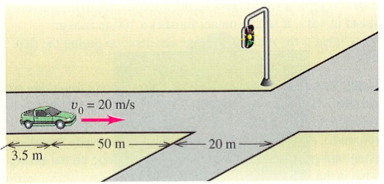
\includegraphics[scale=.85]{/Users/jgates/desktop/latex/pics/redlight.png}


\vfill
\newpage